\section{Double DQN}
\begin{frame}{}
    \LARGE Reinforcement Learning: \textbf{Double DQN}
\end{frame}

\begin{frame}{Double DQN}
    \textbf{The problem.} Even with a target network, the target computation still has a flaw:
    \begin{equation*}
        y = r + \gamma \max_{a'} \hat{Q}(s', a'; \theta^-)
    \end{equation*}
    The target network both \emph{selects} the best next action (via $\max$) and \emph{scores} it (via $\hat{Q}$) in one step. Taking a max over noisy estimates will almost always pick an overestimated action---and then that overestimate becomes the training target.

    \pause
    \vspace{0.5em}
    \textbf{The fix.} Double DQN splits the job between the two networks we already have:
    \begin{equation*}
        y = r + \gamma\, \hat{Q}\!\left(s',\; \arg\max_{a'} Q(s', a'; \theta);\; \theta^- \right)
    \end{equation*}
    The \textbf{online network} $\theta$ picks which action looks best. The \textbf{target network} $\theta^-$ scores that action. Because their weights differ, their errors do not overlap---overestimation bias is reduced. This is a one-line change to the DQN code.
\end{frame}

\begin{frame}{Target Network vs.\ Double DQN}
    Both use two networks, which makes them easy to confuse. They solve completely different problems:

    \vspace{0.5em}
    \begin{table}[]
        \centering
        \renewcommand{\arraystretch}{2.0}
        \begin{tabular}{>{\raggedright\arraybackslash}p{2.5cm} >{\raggedright\arraybackslash}p{3.8cm} >{\raggedright\arraybackslash}p{4.5cm}}
            \hline
            & \textbf{Problem solved} & \textbf{How} \\
            \hline
            Target Network & Unstable, moving target & Freeze weights for $C$ steps \\
            Double DQN & Overestimation bias & Split action selection from evaluation \\
            \hline
        \end{tabular}
    \end{table}

    \vspace{0.5em}
    The two-network structure was already there from the Target Network. Double DQN just changes \emph{how} those two networks are used.
\end{frame}

\begin{frame}{DDQN Algorithm}
    \begin{figure}
        \centering
        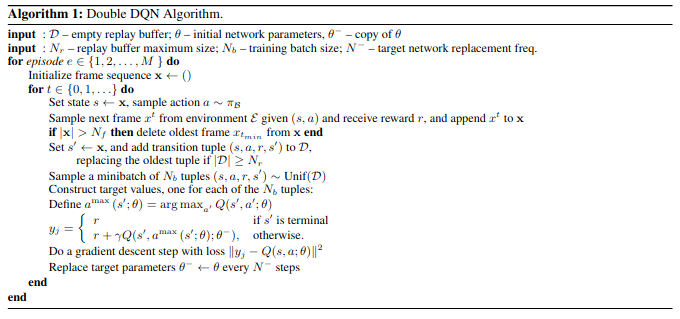
\includegraphics[width=\textwidth,height=0.9\textheight,keepaspectratio]{images/dqn+sarsa/ddqn.png}
    \end{figure}
    \footnotetext{Van Hasselt, Guez \& Silver, \emph{Deep Reinforcement Learning with Double Q-learning}, AAAI 2016}
\end{frame}